\documentclass{article}

\usepackage{tikz}
\usetikzlibrary {positioning}

\begin{document}

1. shifting part: dimension.

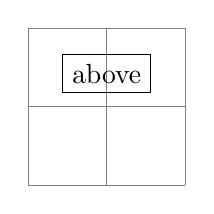
\begin{tikzpicture}
  \draw[help lines] (0,0) grid (2,2);
  \node at (1,1) [above=2pt+3pt,draw] {above};
\end{tikzpicture}

2. shifting part: number.

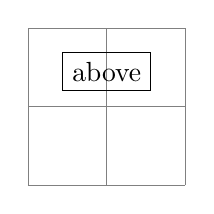
\begin{tikzpicture}
  \draw[help lines] (0,0) grid (2,2);
  \node at (1,1) [above=.2,draw] {above};
  % south border of the node is now 2mm above (1,1)
\end{tikzpicture}

3. shifting part: number-or-dimension-1 and number-or-dimension-2.

\usetikzlibrary {positioning}
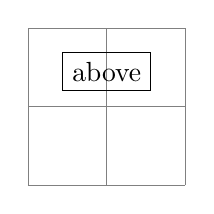
\begin{tikzpicture}
  \draw[help lines] (0,0) grid (2,2);
  \node at (1,1) [above=.2 and 3mm,draw] {above};
  % south border of the node is also 2mm above (1,1)
\end{tikzpicture}

1. of-part: coordinate

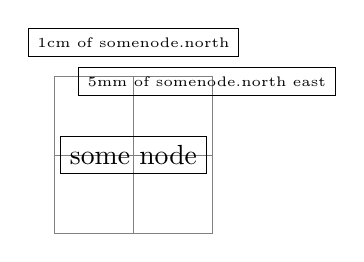
\begin{tikzpicture}[every node/.style=draw]
  \draw[help lines] (0,0) grid (2,2);
  \node (somenode) at (1,1) {some node};

  \node [above=5mm of somenode.north east] {\tiny 5mm of somenode.north east};
  \node [above=1cm of somenode.north]      {\tiny 1cm of somenode.north};
\end{tikzpicture}

2. of-part: node name

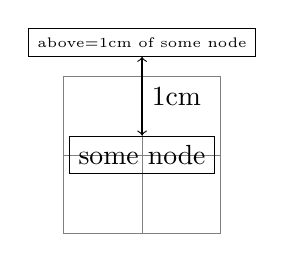
\begin{tikzpicture}[every node/.style=draw]
  \draw[help lines] (0,0) grid (2,2);
  \node (some node) at (1,1) {some node};

  \node (other node) [above=1cm of some node] {\tiny above=1cm of some node};

  \draw [<->] (some node.north) -- (other node.south)
                                node [midway,right,draw=none] {1cm};
\end{tikzpicture}

grid

\usetikzlibrary {positioning}
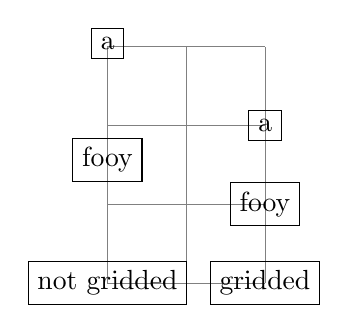
\begin{tikzpicture}[every node/.style=draw]
  \draw[help lines] (0,0) grid (2,3);

  % Not gridded
  \node (a1) at (0,0) {not gridded};
  \node (b1) [above=1cm of a1] {fooy};
  \node (c1) [above=1cm of b1] {a};

  % gridded
  \node (a2) at (2,0) {gridded};
  \node (b2) [on grid,above=1cm of a2] {fooy};
  \node (c2) [on grid,above=1cm of b2] {a};
\end{tikzpicture}

node distance

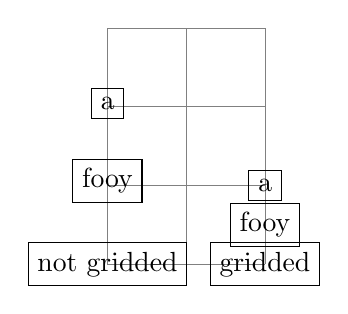
\begin{tikzpicture}[every node/.style=draw,node distance=5mm]
  \draw[help lines] (0,0) grid (2,3);

  % Not gridded
  \node (a1) at (0,0) {not gridded};
  \node (b1) [above=of a1] {fooy};
  \node (c1) [above=of b1] {a};

  % gridded
  \begin{scope}[on grid]
    \node (a2) at (2,0) {gridded};
    \node (b2) [above=of a2] {fooy};
    \node (c2) [above=of b2] {a};
  \end{scope}
\end{tikzpicture}

\end{document}
